\documentclass{article}
\usepackage[T1]{fontenc}
\usepackage{lmodern}
\usepackage{graphicx}
\usepackage{amsmath,amssymb}
\usepackage[a4paper,margin=2cm]{geometry}
\usepackage[absolute,overlay]{textpos}
\setlength{\TPHorizModule}{1mm}
\setlength{\TPVertModule}{1mm}
\usepackage[indonesian]{babel}
\usepackage{hyperref}
\setlength{\emergencystretch}{2em}
% unit: Halaman 26

\begin{document}

% === Halaman 26 (llm) ===

\vspace{193.05mm}

Contoh lain:\
Cipherteks: PHHW PH DIWHU WKH WRJD SDUWB

% deskripsi: Ilustrasi proses dekripsi Caesar Cipher dengan mencoba berbagai nilai kunci (k) untuk menerjemahkan cipherteks menjadi plaintext yang terbaca.
% bbox normalisasi: [0.0900, 0.2000, 0.5600, 0.8500]
\begin{textblock*}{98.70mm}(18.90mm,59.40mm)
\noindent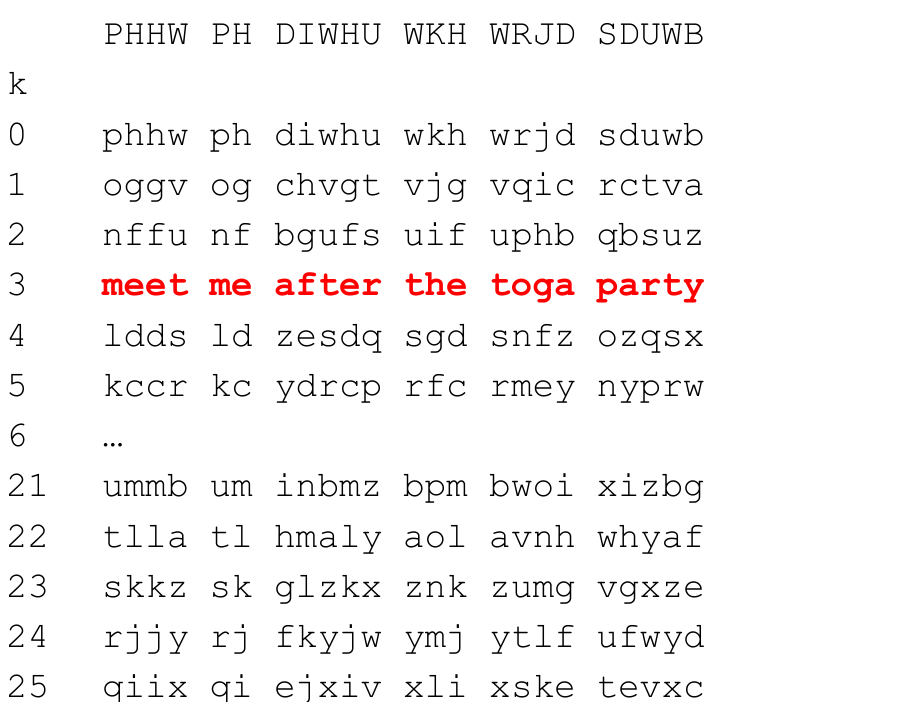
\includegraphics[width=98.70mm,height=193.05mm]{../../images/llm/page_026_img_01.png}%
\end{textblock*}

\end{document}
